% concatenated from paper_square_v2.tex
% !TeX program = pdflatex
\documentclass[11pt,a4paper]{article}

\usepackage[utf8]{inputenc}
\usepackage[T1]{fontenc}
\usepackage{lmodern}
\usepackage{amsmath,amssymb,amsthm}
\usepackage{mathtools}
\usepackage{geometry}
\usepackage{graphicx}
\usepackage{booktabs}
\usepackage{caption}
\usepackage{hyperref}
\usepackage{enumitem}
\usepackage{cleveref}
\usepackage{xcolor}
\usepackage{csquotes}
\usepackage{pgfplots}
\pgfplotsset{compat=1.18}
\usepackage{listings}
\lstset{
  basicstyle=\ttfamily\small,
  columns=fullflexible,
  breaklines=true,
  keepspaces=true,
  showstringspaces=false
}

\usepackage[backend=biber,
style=numeric,
sorting=nyt,
giveninits=true,
doi=false,
isbn=false,
url=false,
eprint=false,
maxbibnames=99]{biblatex}

\usepackage[framemethod=tikz]{mdframed}
\mdfsetup{
  backgroundcolor=gray!5,
  linecolor=gray!50,
  linewidth=0.8pt,
  roundcorner=4pt,
  skipabove=1em,
  skipbelow=1em,
  innerleftmargin=10pt,
  innerrightmargin=10pt,
  innertopmargin=8pt,
  innerbottommargin=8pt
}

\usepackage{tikz}
\usetikzlibrary{arrows.meta,positioning,fit,calc, backgrounds}

% needed for pgfonlayer
\pgfdeclarelayer{background}
\pgfsetlayers{background,main}


\newcommand{\tikzmark}[1]{%
  \tikz[remember picture,overlay]\coordinate (#1);%
}

\addbibresource{literature.bib}


\geometry{margin=1in}

\newcounter{todo}
\setcounter{todo}{0}

\newcommand{\todo}[1]{%
  \refstepcounter{todo}%
  \textbf{\textcolor{red}{[TODO~\thetodo: #1]}}%
}

\newcommand{\listtodos}{%
  \textbf{Total TODOs: \thetodo}%
}

\newcommand{\st}{%
  \text{\qquad s.t.\qquad}%
}


\theoremstyle{plain}
\newtheorem{theorem}{Theorem}
\newtheorem{lemma}{Lemma}
\newtheorem{proposition}{Proposition}
\newtheorem{corollary}{Corollary}

\theoremstyle{definition}
\newtheorem{definition}{Definition}
\newtheorem{problem}{Problem}

\theoremstyle{remark}
\newtheorem{remark}{Remark}

\DeclareMathOperator{\N}{\mathbb{N}}
\DeclareMathOperator{\R}{\mathbb{R}}

\title{From Computational Certification to Exact Coordinates:\\
Heilbronn's Triangle Problem on the Unit Square\\
Using Mixed-Integer Optimization}
\author{Nathan Sudermann-Merx\thanks{Institute for Computer Science, DHBW Mannheim. Email: \texttt{nathan.sudermann-merx@dhbw.de}}}
\date{\today}

\begin{document}

\maketitle

\begin{abstract}
  We develop a mixed-integer nonlinear programming (MINLP) approach for the classical Heilbronn triangle problem, demonstrating the capability of modern global optimization solvers to tackle 
  challenging combinatorial geometry problems. A symmetry-breaking strategy based on boundary structure yields a substantially stronger model: for $n=9$, we compute an $\varepsilon$-globally optimal 
  point in 15 minutes on a standard desktop computer, improving upon the previously reported effort of approximately one day. By combining numerical certification with exact symbolic computation, 
  we recover exact coordinates matching all best-known configurations for $n\le 9$, including the $n=9$ configuration of Comellas and Yebra (2002). 
  An analysis of these configurations reveals the clustering of noncritical triangle areas around a small number of distinct values, suggesting rich underlying algebraic structure. 
  All code and data are publicly available.
  \end{abstract}
    
\section{Introduction}

\subsection{The problem}

The Heilbronn triangle problem arises in discrete geometry and asks:

\begin{mdframed}
  \centering
  \emph{How should $n$ points be placed in the unit square so that the smallest triangle determined by any three of them is as large as possible?}
  \end{mdframed}

  The problem is named after the mathematician Hans Heilbronn (and not after the city in southern Germany), who was born into a German-Jewish family and left Germany in 1933 during the rise of the Nazi regime. It first appeared in print in Roth's 1951 paper~\cite{Roth1951}, where the unit square was replaced by an arbitrary closed convex region in the plane of positive measure, and the emphasis was placed on the asymptotic behavior of the minimal triangle area rather than on explicit constructions for small values of $n$.

\subsection{Upper bounds}

We denote the minimal triangle area in an optimal configuration of $n$ points in the unit square by $\Delta_n$.
Heilbronn conjectured that $\Delta_n$ should satisfy an asymptotic upper bound of the form
\[
\Delta_n = O\!\left(\frac{1}{n^2}\right).
\]
As we will see in Section~\ref{sec: lower bounds}, this turned out to be incorrect.
Roth observed in~\cite{Roth1951} that the problem admits a simple upper bound,
\[
\Delta_n \le \frac{1}{n-2}.
\]
To see this, note that the convex hull of any configuration of $n$ points can be partitioned into $n-2$ triangles with pairwise disjoint interiors and total area at most $1$, implying that at least one of these triangles must have area no greater than $1/(n-2)$.
Over the following decades, the upper bounds were steadily refined. In 1972, Schmidt~\cite{Schmidt1972} obtained a significant improvement, which was sharpened by Roth~\cite{Roth1972II,Roth1972III} later that year and further strengthened by Koml\'os, Pintz, and Szemer\'edi~\cite{KPS1981} in 1981, establishing what remained the best-known estimate for over forty years.
A major breakthrough came in 2023, when Cohen, Pohoata, and Zakharov~\cite{CPZ2023} proved that for all sufficiently large $n$,
\[
\Delta_n \le n^{-8/7 - 1/2000},
\]
which is currently the strongest known asymptotic upper bound. Figure~\ref{fig:CPZbound} illustrates that this bound provides a reasonably tight envelope for all best-known configurations with $n \ge 6$.

\begin{figure}[h]
  \centering
  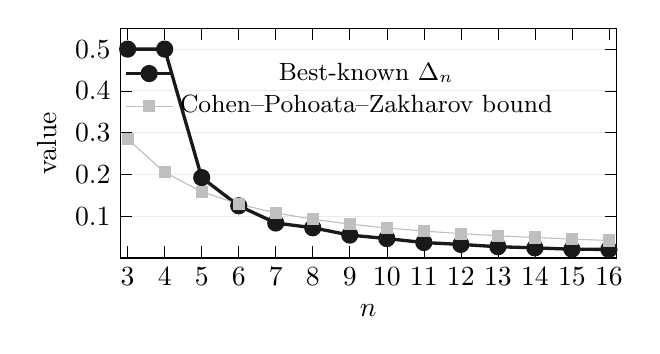
\begin{tikzpicture}
  \begin{axis}[
      width=0.65\linewidth,
      height=4.5cm,
      xlabel={$n$},
      ylabel={value},
      xmin=2.8, xmax=16.2,
      ymin=0, ymax=0.55,
      xtick={3,4,...,16},
      ytick={0.1,0.2,...,0.5},
      ymajorgrids,
      grid style={gray!15},
      axis line style={black},
      tick style={black},
      legend style={
          at={(0.9,0.9)},
          anchor=north east,
          draw=none,
          fill=none,
          font=\small
      },
  ]
  
  % Best-known Δ_n
  \addplot[
      very thick,
      gray!20!black,
      mark=*,
      mark size=2.5pt
  ] coordinates {
  (3,0.5)
  (4,0.5)
  (5,{sqrt(3)/9})
  (6,{1/8})
  (7,0.0838)
  (8,{(sqrt(13)-1)/36})
  (9,{(9*sqrt(65)-55)/320})
  (10,0.0465)
  (11,{1/27})
  (12,0.0325)
  (13,0.0270)
  (14,0.0243)
  (15,0.0211)
  (16,{7/341})
  };
  \addlegendentry{Best-known $\Delta_n$}
  
  % CPZ bound
  \addplot[
      thin,
      gray!50,
      mark=square*,
      mark size=2pt
  ] coordinates {
  (3,{pow(3,-(8/7+1/2000))})
  (4,{pow(4,-(8/7+1/2000))})
  (5,{pow(5,-(8/7+1/2000))})
  (6,{pow(6,-(8/7+1/2000))})
  (7,{pow(7,-(8/7+1/2000))})
  (8,{pow(8,-(8/7+1/2000))})
  (9,{pow(9,-(8/7+1/2000))})
  (10,{pow(10,-(8/7+1/2000))})
  (11,{pow(11,-(8/7+1/2000))})
  (12,{pow(12,-(8/7+1/2000))})
  (13,{pow(13,-(8/7+1/2000))})
  (14,{pow(14,-(8/7+1/2000))})
  (15,{pow(15,-(8/7+1/2000))})
  (16,{pow(16,-(8/7+1/2000))})
  };
  \addlegendentry{Cohen--Pohoata--Zakharov bound}
  
  \end{axis}
  \end{tikzpicture}
  \caption{Best-known values of $\Delta_n$ for the Heilbronn problem in the unit square compared with the asymptotic upper bound $n^{-8/7-1/2000}$ of Cohen, Pohoata, and Zakharov~\cite{CPZ2023}.}
  \label{fig:CPZbound}
  \end{figure}

\subsection{Lower bounds}\label{sec: lower bounds}

A simple lower bound of order $c/n^3$ for $\Delta_n$ can be obtained as follows. 
Without regard to the unit-square constraint, consider the $n$ points $(i,i^2)$ for $i=0,\ldots,n-1$. 
No three of these points are collinear, and hence every triangle determined by them has strictly positive area. 
Moreover, each triangle area can be expressed as half the absolute value of a $3\times 3$ determinant formed from the vertices' coordinates (see Section~\ref{sec:original formulation}). 
Since all coordinates are integers and the area is positive, the determinant has absolute value at least $1$, implying that every triangle has area at least $1/2$.
To place the configuration inside the unit square, scale the $x$-coordinates by $1/n$ and the $y$-coordinates by $1/n^2$. 
Areas then scale by $1/n^3$, giving
\[
\Delta_n \ge \frac{1}{2n^3}.
\]
As noted in the appendix of Roth's paper~\cite{Roth1951}, Paul Erd\H{o}s refined this idea by choosing a prime $p$ with $n \le p \le 2n$ and considering the points $(i, i^2 \bmod p)$ for $i=0,\ldots,p-1$. 
This construction preserves the key properties used above—integral coordinates and the absence of collinear triples—while having the advantage that the $y$-coordinates are bounded by $p$. 
Consequently, scaling to the unit square reduces areas only by a factor of $1/p^2$, leading to
\[
\Delta_n \ge \frac{1}{2p^2} \ge \frac{1}{8n^2}
\]
for all $n$.

Combined with Heilbronn's conjecture, this would have yielded the correct asymptotic order of magnitude for the problem. 
However, in 1982, following a suggestion by Roth that the conjecture might be false, Koml\'os, Pintz, and Szemer\'edi proved in~\cite{KPS1982} that there exists a constant $c>0$ such that
\[
\Delta_n \ge \frac{c \log n}{n^2}
\]
for infinitely many $n$, using a nonconstructive probabilistic argument. 
This gap between existence and construction was closed in 2000 by Bertram-Kretzberg, Hofmeister, and Lefmann~\cite{BHL2000}, who presented a polynomial-time algorithm producing configurations with asymptotic lower bound $\Omega(\log n/n^2)$.


\subsection{Results for small-$n$-configurations}

All best-known configurations for the Heilbronn problem with $n \le 16$ are documented on \emph{Erich's Packing Center}, a website maintained by Erich Friedman that tracks records for a variety of computational geometry problems (see~\cite{FriedmanPackingCenter}).
The first case requiring a nontrivial proof, $n=5$, was resolved in 1991 by Yang, Zhang, and Zeng~\cite{yzz91}, who proved
$\Delta_5 = \sqrt{3}/9$.
In the same work, they disproved a conjecture of Goldberg, who had suggested that optimal configurations for $n \le 7$ arise from affine images of regular $n$-gons—a statement that turns out to hold only for $n=6$.
In 1995, Dress, Yang, and Zeng~\cite{dyz1995} established the optimal value $\Delta_6 = 1/8$.

In 2002, Comellas and Yebra~\cite{comellasyebra2002} used simulated annealing followed by an analytical refinement procedure to discover best-known configurations and exact coordinates for many cases with $n \le 12$.
As we shall see, their configurations for $n=7,8,9$ have since all been proved optimal, and their configurations for $n=10$ and $n=12$ remain the best known to date.
The optimality of their configuration for $n=7$, with $\Delta_7 \approx 0.083859$, was proved in 2011 by Zeng and Chen~\cite{ZengChen2011}, who decomposed the problem into 226 nonlinear optimization subproblems.
For $n=9$, Chen, Xu, and Zeng~\cite{chen2017searching} conducted in 2017 an extensive branch-and-bound computation using CPU and GPU clusters, requiring a total of 125 days of wall-clock time to obtain sharp upper bounds.
In 2022, Dehbi and Zeng~\cite{dehbi2022heilbronn} combined numerical search with symbolic computation to prove that the configuration for $n=8$ found by Comellas and Yebra, satisfying
$\Delta_8 = (\sqrt{13}-1)/36$,
is indeed optimal.

For $n \ge 13$, the best-known configurations were found by Peter Karpov ($n=13,15$) and Mark Beyleveld ($n=14,16$) but have not been formally published; they are available 
only through personal communication with Erich Friedman and are presented in Appendix~\ref{app:best-known}.

More recently, in 2025, Monji, Modir, and Kocuk~\cite{monji2025solvingheilbronntriangleproblem} applied nonlinear global optimization techniques to compute an optimality certificate for $\Delta_9$, reducing the total wall-clock time to approximately one day using a state-of-the-art mixed-integer solver.

These results illustrate a broader trend: modern mixed-integer nonlinear programming (MINLP) solvers have matured to the point where they can tackle geometric 
optimization problems that were out of reach for general-purpose methods only a decade ago. Recent systematic studies by Berthold et al.~\cite{berthold2026global,berthold2026outoftheboxglobaloptimizationpacking}
confirm this observation across a range of combinatorial geometry problems, showing that straightforward MINLP formulations solved with off-the-shelf solvers 
can match or improve upon the best previously known solutions.  The present paper continues this line of work for the Heilbronn problem. 

\subsection{Contributions}

The contributions of this paper are fourfold.

\paragraph{A stronger mixed-integer formulation.}
We develop a mixed-integer optimization model for the Heilbronn problem that incorporates a novel symmetry-breaking strategy based on the boundary structure of optimal configurations.  This strategy fixes several point coordinates a~priori and, in addition, determines the orientation of certain triangles, which allows us to fix a number of binary sign variables before the solve.
Together, these reductions lead to a formulation that is substantially stronger than existing models.  In particular, the Heilbronn problem for $n=9$ can be solved to certified global optimality in approximately 15 minutes on a standard desktop computer, improving upon the previously reported effort of about one day~\cite{monji2025solvingheilbronntriangleproblem} by more than an order of magnitude.

\paragraph{Exact coordinates via an optimize-then-refine framework.}
We introduce a two-step methodology that combines global optimization (Step~1) with exact symbolic refinement (Step~2).  The numerical solution from the solver identifies the 
combinatorial structure of an optimal configuration---specifically, which triangles are critical and which points lie on the boundary.  This information yields a structured 
polynomial system that is then solved exactly using computer algebra.  Applying this pipeline, we derive closed-form exact coordinates for all optimal configurations 
with $n = 5, \ldots, 9$, confirming earlier results of Comellas and Yebra~\cite{comellasyebra2002} and sometimes simplifying their presentation.
\paragraph{Structural observations and new research questions.}
An empirical analysis of the certified optimal configurations reveals two notable patterns: the number of critical triangles grows steadily with $n$, and the areas of the noncritical triangles cluster into a small number of distinct values.  We document these observations and pose them as open research questions that may guide future investigations into the combinatorial geometry of extremal point sets.

\paragraph{Reproducibility and data.}
Many of the best-known configurations for the Heilbronn problem have circulated only through personal communication rather than formal publication, making independent verification difficult.  We collect all best-known configurations for $n \le 16$ in this paper and its appendix.
The complete source code, input data, and resulting solution files are publicly
available at \url{https://github.com/spiralulam/heilbronn}.

\subsection{Paper outline}

Section~\ref{sec:formulation} establishes a formal setting for the Heilbronn problem and derives structural properties of optimal configurations that are exploited in the optimization model.
Section~\ref{sec:MIPModel} develops the mixed-integer formulation and its enhancements, including a symmetry-breaking strategy based on the boundary structure of optimal configurations.
Section~\ref{sec:framework} presents the optimize-then-refine framework and illustrates it in detail for $n=7$.
Section~\ref{sec:solutions} reports the exact coordinates for $n = 5, \ldots, 9$.
Section~\ref{sec:observations} discusses the structural patterns and open questions.
Section~\ref{sec:outlook} concludes with an outlook.
Appendix~\ref{app:best-known} collects the best-known configurations for $n = 10, \ldots, 16$.

\section{Original formulation and theoretical results}\label{sec:formulation}

This section establishes a basic formulation of the Heilbronn problem in Section~\ref{sec:original formulation}, which already suffices to prove its solvability.
The theoretical results in Section~\ref{sec: boundary configuration} about the boundary points of optimal configurations and in Section~\ref{sec: triangle sign}
about a sign property of determinants are not only of theoretical interest but provide valuable structure that is exploited in the optimization model of Section~\ref{sec:MIPModel}, leading to a substantial runtime reduction.

\subsection{The original formulation and its solvability}\label{sec:original formulation}

Let $n\ge 3$ denote the number of points $p_1=(x_1,y_1),\ldots,p_n=(x_n,y_n)$ we want to place in $\R^2$, $I=\{1,\ldots,n\}$, and 
\[
T\ =\ \{(i,j,k)|\ 1\le i<j<k\le n\}\subset \N^3
\]
the set of all triangles, where each triangle $t=(i,j,k)\in T$ is identified with the indices of the defining points $p_i$, $p_j$ and $p_k$.
By construction, $|T|=\binom{n}{3}$.
\begin{remark}
  The enumeration of the points heavily influences the symmetry breaking and therefore 
   becomes a crucial modeling choice, as discussed in Section~\ref{sec: symmetry breaking}.
\end{remark}

Further, let $A_t$ be the area of triangle $t$ and $[0,1]^2$ the unit square. Then the Heilbronn problem can be formulated as the following optimization problem:
\[
P_\Delta:\qquad
\max_{x,y}\ \min_{t\in T} A_t
\quad
\text{s.t. } (x_i,y_i)\in[0,1]^2,\ i\in I.
\]
and $\Delta_n$ coincides with the optimal value of $P_\Delta$.
All further specifications of this problem amount to modeling decisions, of which there are many and which must be made carefully. A first fundamental modeling choice concerns the representation of the triangle areas. 
For a triangle $t=(i,j,k)$, the area can be expressed via the classical shoelace determinant formula,
\[
A_t
= \frac{1}{2}\left|\det
\begin{pmatrix}
x_i & y_i & 1\\
x_j & y_j & 1\\
x_k & y_k & 1
\end{pmatrix}
\right|
=
\frac{1}{2}
\left|
x_i y_j + x_j y_k + x_k y_i
-
x_i y_k - x_j y_i - x_k y_j
\right|.
\]

With this representation, $P_\Delta$ becomes a nonsmooth, nonconvex optimization problem with box constraints with the following properties.

\begin{proposition}\label{prop:solvability-positive-optval}
  The optimization problem $P_\Delta$ admits a solution for every $n$, and its optimal value $\Delta_n$ is strictly positive.
  \end{proposition}
  
  \begin{proof}
  Existence of a solution follows from the Weierstraß theorem. 
  The objective function is continuous, and the feasible set is nonempty, closed, and bounded; hence it is compact. 
  Therefore, the maximum is attained. Strict positivity of $\Delta_n$ follows, for example, from Erd\H{o}s' construction discussed in Section~\ref{sec: lower bounds}, which provides an explicit positive lower bound.
  \end{proof}
  
  \begin{remark}
  In~\cite{Roth1951}, Roth argues that $P_\Delta$ is solvable because its feasible set \enquote{is a closed convex region}. 
  However, closedness and convexity alone do not guarantee existence of a maximizer; compactness (or an equivalent coercivity argument) is required.
  \end{remark}
  
  The following corollaries are immediate consequences of Proposition~\ref{prop:solvability-positive-optval}, since otherwise the configuration would contain a triangle of zero area.

  \begin{corollary}
  An optimal configuration for the Heilbronn problem does not contain two coincident points.
  \end{corollary}
  
  \begin{corollary}
  An optimal configuration for the Heilbronn problem does not contain three collinear points.
  \end{corollary}

\subsection{Boundary structure of optimal configurations}\label{sec: boundary configuration}

Let $P=\{p_1,\dots,p_n\}\subseteq S=[0,1]^2$ be an optimal configuration
for the Heilbronn problem, and let
\[
K := \operatorname{conv}(P)
= \Bigl\{\sum_{i=1}^{n}\lambda_i\, p_i \;\Big|\; \lambda_i\ge 0,\;\sum_{i=1}^{n}\lambda_i=1\Bigr\}
\]
denote its convex hull.
Let $v_1,\dots,v_m$ be the vertices of $K$, listed in cyclic order,
so that $K = v_1 v_2 \cdots v_m$ is a convex $m$-gon.

\begin{lemma}[Minimal covering parallelogram]\label{lem:min_parallelogram}
The unit square $S=[0,1]^2$ is a minimum-area covering parallelogram of $K$.
\end{lemma}

\begin{proof}
Assume for contradiction that there exists a parallelogram $S' \supseteq K$
with $\operatorname{area}(S') < 1$.

Since every parallelogram is an affine image of the unit square,
there exists an affine bijection $T: S' \to S$
with positive determinant satisfying
\[
|\det T| = \frac{\operatorname{area}(S)}{\operatorname{area}(S')}
= \frac{1}{\operatorname{area}(S')} > 1.
\]

Because $K \subseteq S'$, we have $T(K) \subseteq S$, hence $T(P) \subseteq S$.
For every triangle $\tau$ formed by points of $P$,
its area scales by
\[
\operatorname{area}(T(\tau))
= |\det T| \operatorname{area}(\tau).
\]
Thus
\[
\Delta(T(P))
= |\det T| \Delta(P)
> \Delta(P),
\]
contradicting the optimality of $P$.
\end{proof}

\begin{proposition}\label{thm:boundary_vertices}
Let $n\ge 5$ and let $P\subseteq[0,1]^2$ be an optimal configuration.
Then at least five distinct vertices of $K=\operatorname{conv}(P)$
lie on the boundary $\partial S$ of the unit square.
\end{proposition}

\begin{proof}
By Lemma~\ref{lem:min_parallelogram}, $S$ is a minimum-area covering parallelogram of $K$.
Applying Lemma~2 of Zeng and Chen~\cite{ZengChen2011} yields three possible cases:

\begin{enumerate}
\item \textbf{No common vertices.}
Then at least five vertices of $K$ lie on the four edges of $S$.

\item \textbf{Exactly one common vertex.}
Then each adjacent edge interior contains a vertex of $K$,
and the remaining two edges each contain a vertex,
yielding at least five distinct boundary vertices.

\item \textbf{Two common vertices forming a diagonal.}
Then each of the four edges of $S$ contains a vertex of $K$
in its interior.
Together with the two corner vertices,
this yields at least six distinct boundary vertices.
\end{enumerate}

In all cases, $\partial S$ contains at least five distinct vertices of $K$,
hence at least five distinct points of $P$.
\end{proof}

\begin{remark}
  The argument of this subsection is essentially due to Amirali Modir, who
  communicated to us the proof of Proposition~\ref{thm:boundary_vertices}
  building on Lemma~2 of Zeng and Chen~\cite{ZengChen2011}. Our only
  contribution is Lemma~\ref{lem:min_parallelogram}, which shows that the unit
  square is a minimum-area covering parallelogram of the convex hull and thereby
  makes the result of Zeng and Chen directly applicable in our setting.
\end{remark}

\subsection{On the signs of the triangle areas}\label{sec: triangle sign}

The signed area of a triangle with vertices $p_i,p_j,p_k$ is
\[
  A^\pm(i,j,k)
  :=\frac{1}{2}\det\!\begin{pmatrix}
  1 & x_i & y_i\\
  1 & x_j & y_j\\
  1 & x_k & y_k
  \end{pmatrix}
  =\frac{1}{2}\bigl[(x_j-x_i)(y_k-y_i)-(y_j-y_i)(x_k-x_i)\bigr].
\]
It is well known that $A^\pm(i,j,k)>0$ if and only if $(p_i,p_j,p_k)$ are ordered counterclockwise,
$A^\pm(i,j,k)<0$ for a clockwise ordering, and $A^\pm(i,j,k)=0$ for collinear points.
In particular, the (unsigned) area satisfies $A(i,j,k)=|A^\pm(i,j,k)|$,
and for counterclockwise-ordered triples $A(i,j,k)=A^\pm(i,j,k)$.
This sign information plays a key role in the optimization model of Section~\ref{sec:MIPModel}.

\section{Mixed-integer optimization models}\label{sec:MIPModel}

In Section~\ref{sec:MIPmodelVanilla} we present a baseline mixed-integer formulation that mirrors the original nonsmooth model as closely as possible; solving this model already certifies optimality for small instances but becomes intractable around $n=8$.
Section~\ref{sec:MIPmodelImproved} then develops several enhancements---in particular a symmetry-breaking strategy based on boundary structure that, as a byproduct, also fixes the signs of certain triangle areas.
Together, these improvements lead to a much stronger formulation.
The resulting final model is collected in Section~\ref{sec:final-model}, and Section~\ref{sec:comparison-monji} compares it with the formulation of Monji, Modir, and Kocuk~\cite{monji2025solvingheilbronntriangleproblem}.

\subsection{A first mixed-integer formulation}\label{sec:MIPmodelVanilla}

For each triangle $t=(i,j,k) \in T$ we introduce a continuous auxiliary variable
$A_t^{\pm} \in [-\tfrac{1}{2}, \tfrac{1}{2}]$ representing the signed area
\[
A_t^{\pm}
=
\frac{1}{2}\left(
x_i y_j + x_j y_k + x_k y_i
-
x_i y_k - x_j y_i - x_k y_j
\right).
\]
To eliminate the minimum over triangles in the objective, we introduce an auxiliary variable
$z$ and impose
\[
z \le |A_t^{\pm}|, \qquad t \in T.
\]
This formulation remains nonsmooth because of the absolute value.
To handle it, we introduce a binary variable $b_t\in\{0,1\}$ for each triangle $t$
that selects the sign of $A_t^{\pm}$,
and replace the absolute-value constraint by
\[
z \le (2b_t - 1)\, A_t^{\pm}, \qquad t \in T.
\]
Maximizing $z$ forces the model to choose the sign that yields the larger of $-A_t^\pm$ and $A_t^\pm$, thereby mimicking the absolute value 
$|A_t^\pm|=\max(A_t^\pm,-A_t^\pm)$.

Our first baseline mixed-integer optimization model is therefore

\begin{align*}
P_\Delta^0:\qquad
\max_{z,x,y}\quad & z \\
\text{s.t.}\quad 
& (x_i,y_i)\in[0,1]^2, \quad i\in I,\\
& A_t^{\pm}
=
\frac{1}{2}\left(
x_i y_j + x_j y_k + x_k y_i
-
x_i y_k - x_j y_i - x_k y_j
\right), 
\quad t\in T,\\
& z \le (2b_t - 1)\, A_t^{\pm}, \quad t\in T,\\
& A_t^{\pm}\in\left[-\frac{1}{2}, \frac{1}{2}\right],\\
& b_t \in \{0,1\}, \quad t\in T,\\
&  0 \le z \le \frac{1}{2}.
\end{align*}

This formulation is a nonlinear mixed-integer model
and can in principle be solved by any MINLP solver.

\begin{remark}
This baseline model solves the case $n=5$ within seconds using Gurobi and 
proves optimality for $n=6$ in approximately three minutes.
For $n=7$, however, the solver did not terminate within 45 minutes,
illustrating the rapid growth in computational difficulty.
\end{remark}

\subsection{Some improvements}\label{sec:MIPmodelImproved}

We enhance the baseline model with three key improvements.

\subsubsection{Bounds and variable substitution}

We add the constraint $z \le \Delta_{n-1}$ (since solving the problem for $n-1$ points provides an upper bound for $n$ points). Additionally, we introduce auxiliary variables $w_{ij} \in [0,1]$ with $w_{ij} = x_i y_j$ to isolate bilinear terms, which are the main source of nonconvexity and are approximated by solvers using techniques such as McCormick inequalities.

\subsubsection{Symmetry breaking}\label{sec: symmetry breaking}

The primary obstacle is the enormous symmetry: the dihedral group $D_4$ acts on coordinates (8 symmetries: 4 rotations, 4 reflections) and the symmetric group $S_n$ permutes point labels, yielding a combined symmetry group of order $8 \cdot n!$. For $n=9$, this is up to 2.9 million equivalent solutions. 
Our strategy exploits the boundary structure of optimal configurations using Proposition~\ref{thm:boundary_vertices} to break this symmetry in three steps:

\paragraph{Step 1: Boundary assignment and elimination of geometric symmetry.}
We designate the edge carrying at least two boundary vertices as the left edge ($x = 0$), eliminating all rotations in $D_4$. Combined with the constraint $x_2 \le x_4$, this breaks all reflection symmetries.

\paragraph{Step 2: Canonical boundary labeling.}
We label the five boundary points $p_1, \ldots, p_5$ counterclockwise starting from the left edge, assigning them to specific edges: $p_1$ (left, lower), $p_2$ (bottom), $p_3$ (right), $p_4$ (top), $p_5$ (left, upper). The constraint $y_5 \ge y_1$ resolves ambiguity among left-edge points.

\paragraph{Step 3: Interior point ordering.}
The remaining points $p_6, \ldots, p_n$ are ordered by increasing $x$-coordinate, eliminating the $(n-5)!$ labeling symmetries.

This three-step approach fixes five coordinate variables outright and breaks the combined symmetry group, which is crucial for solver performance. 
Table~\ref{tab:fixed-vars} and Figure~\ref{fig:symbreak} illustrate the resulting configuration structure.

\begin{table}[ht]
  \centering
    \begin{tabular}{c c c l}
      \toprule
      Point & Coord.\ & Value & Edge \\
      \midrule
      $p_1$ & $x_1$ & $0$ & left \\
      $p_2$ & $y_2$ & $0$ & bottom \\
      $p_3$ & $x_3$ & $1$ & right \\
      $p_4$ & $y_4$ & $1$ & top \\
      $p_5$ & $x_5$ & $0$ & left \\
      \bottomrule
    \end{tabular}
    \caption{Coordinates fixed a~priori by the symmetry-breaking strategy.
    The remaining free coordinates are $y_1$, $x_2$, $y_3$, $x_4$, $y_5$, and all coordinates of $p_6,\dots,p_n$, subject to $y_5\ge y_1$, $x_2\le x_4$, and $x_6\le\cdots\le x_n$.}
    \label{tab:fixed-vars}
\end{table}

\begin{figure}[ht]
  \centering
  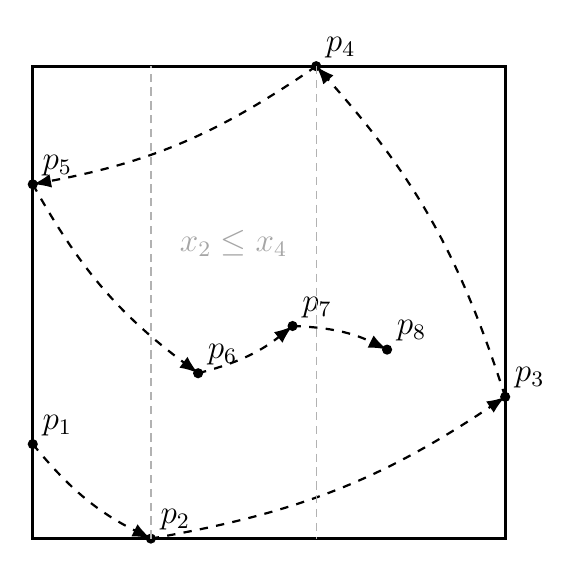
\begin{tikzpicture}[
      scale=6,
      point/.style={circle, fill=black, inner sep=1.3pt},
      lab/.style={font=\large},
      order/.style={-Latex, black, dashed, line width=0.8pt},
      guide/.style={densely dashed, gray!60, line width=0.5pt},
      ineq/.style={gray!70, line width=0.95pt}
  ]
  
  % unit square
  \draw[line width=1pt] (0,0) rectangle (1,1);
  
  \coordinate (p1) at (0,0.20);
  \coordinate (p2) at (0.25,0);
  \coordinate (p3) at (1,0.30);
  \coordinate (p4) at (0.60,1);
  \coordinate (p5) at (0,0.75);
  
  \coordinate (p6) at (0.35,0.35);
  \coordinate (p7) at (0.55,0.45);
  \coordinate (p8) at (0.75,0.4);
  
  \draw[order] (p1) to[bend right=12] (p2);
  \draw[order] (p2) to[bend right=12] (p3);
  \draw[order] (p3) to[bend right=12] (p4);
  \draw[order] (p4) to[bend left=12] (p5);

  \draw[order] (p5) to[bend right=12] (p6);
  
  \draw[order] (p6) to[bend right=12] (p7);
  \draw[order] (p7) to[bend left=12] (p8);
  
  \foreach \i/\p in {1/p1,2/p2,3/p3,4/p4,5/p5,6/p6,7/p7,8/p8}{
      \node[point] at (\p) {};
      \node[lab, anchor=west] at ($(\p)+(0,0.04)$) {$p_{\i}$};
  }
  
  \draw[guide] (p2) -- ($(p2)+(0,1)$);
  \draw[guide] (p4) -- ($(p4)-(0,1)$);
  
\node[font=\large, gray!70] at ($(p2)!0.5!(p4) + (0,0.125)$) {$x_2 \le x_4$};  
\end{tikzpicture}
  
\caption{Symmetry breaking used in the optimization model. 
Five points are fixed on the boundary in counterclockwise order, while the remaining points are ordered by increasing $x$-coordinate; additionally $x_2 \le x_4$.}
\label{fig:symbreak}
\end{figure}

\begin{remark}
  This symmetry-breaking approach also yields correct results for $n<5$, although the theoretical justification does not stem from Proposition~\ref{thm:boundary_vertices}
  but from a separate investigation of the cases $n=3$ and $n=4$. 
\end{remark}

\subsubsection{Sign fixing}

The symmetry breaking approach from Section~\ref{sec: symmetry breaking} allows us to fix the signs for two groups of triangles:
\begin{enumerate}
  \item All triangles in the set $T^+=\{(i,j,k)\in T\mid k\le 5\}$ have their three vertices on the boundary, arranged counterclockwise (since $i<j<k$). Therefore $A_t^\pm\ge 0$ for all $t\in T^+$.
  \item Since $p_1$ and $p_5$ are located on the left edge with $y_5\ge y_1$, we have $A_t^\pm\le 0$ for all $t\in T^-:=\{(i,j,k)\in T\mid i=1,\ j=5\}$.
\end{enumerate}

This allows us to add the constraints
\[
b_t=1,\ t\in T^+\qquad\text{and}\qquad b_t=0,\ t\in T^-
\]
and therefore fix some of the binary variables in advance.
\begin{remark}
  It is also valid to introduce only the binary variables that are not fixed a priori, but we did not experience a computational advantage from that approach.
\end{remark}

  \subsection{Comparison with Monji, Modir, and Kocuk}\label{sec:comparison-monji}

  Concurrent work by Monji, Modir, and Kocuk~\cite{monji2025solvingheilbronntriangleproblem} was the first to apply MINLP solvers to the Heilbronn problem, certifying $n=9$ within one day---a major improvement over prior methods. Our formulation differs in several key respects:
  
\begin{enumerate}
  \item \textbf{Absolute value handling:} We replace $z \le |A_t^\pm|$ with the bilinear constraint $z \le (2b_t-1)A_t^\pm$, avoiding big-$M$ parameters and leveraging the mixed-integer nonlinear programming solver's spatial branching.

  \item \textbf{Symmetry breaking:} We fix five boundary points on specific edges in counterclockwise order eliminating 5 coordinates outright, whereas Monji et~al.\ impose ordering constraints. This also enables sign fixing for $\binom{5}{3} + (n-5)$ binary variables.

  \item \textbf{Minimal auxiliary variables:} We introduce no edge-proximity, strip-assignment, or grid-cell auxiliary binary variables.

  \item \textbf{No pre-processing:} Unlike Monji et~al.\ no optimization-based bound-tightening or other pre-processing techniques are used.
\end{enumerate}

  The result is a more compact model that solves faster (15 minutes for $n=9$ vs.\ one day) without pre-processing.

\subsection{The final model}\label{sec:final-model}

Combining all ingredients from the previous subsection we arrive at the formulation~$P_\Delta^\star$ displayed in Figure~\ref{fig:final-model}.
The colored boxes highlight the individual enhancement groups; the core model corresponds to the baseline formulation~$P_\Delta^0$ expressed in the substituted variables.

  \begin{figure}[h]
    \centering
    
    \begin{align*}
      P_\Delta^\star:\qquad \max_{z,x,y}\quad & z \\[2pt]
      \text{s.t.}\quad
      & \tikzmark{core-tl}(x_i,y_i)\in[0,1]^2,\quad i\in I,\\
      & A_{ijk}^{\pm}\ =\ \frac{1}{2}\left(
        w_{ij} + w_{jk} + w_{ki} - w_{ik} - w_{ji} - w_{kj}
        \right),\quad (i,j,k)\in T\\
      & z\ \le\  (2b_t - 1) A_t^\pm,\quad t\in T\tikzmark{core-br}\\[20pt]
      %
      & \tikzmark{sub-tl}w_{ij}\ =\ x_i y_j,\quad i,j\in I\tikzmark{sub-br}\\[25pt]
      %
      & \tikzmark{sign-tl}b_t=1,\quad t\in T^+\tikzmark{sign-br}\\
      & b_t=0,\quad t\in T^-\\[20pt]
      %
      & \tikzmark{sym-tl}x_1 = x_5 = y_2 = 0\\
      & x_3 = y_4 = 1\\
      & x_2 \le x_4\\
      & y_1 \le y_5\tikzmark{sym-br}\\
      & x_i\ \le\ x_{i+1},\quad i\ge 6\\[20pt]
      %
      & \tikzmark{dom-tl}A_t^{\pm}\in\left[-\frac{1}{2}, \frac{1}{2}\right],\quad t\in T\\
      & w_{ij}\in[0,1],\quad i,j\in I\\
      & b_t \in \{0,1\}, \quad t\in T,\\
      &  0 \le z \le \Delta_{n-1}\tikzmark{dom-br}
    \end{align*}

    
    
    \begin{tikzpicture}[remember picture,overlay]
    \tikzset{
      box/.style={
        rounded corners=2pt,
        inner xsep=6pt,
        inner ysep=4pt,
        line width=0.7pt
      },
      label/.style={
        font=\small\bfseries,
        inner sep=1.5pt,
        rounded corners=2pt
      }
    }

\coordinate (CoreBL) at ($(core-tl |- core-br)+(-100pt,-5pt)$);

\coordinate (CoreTR) at ($(core-br)+(180pt,80pt)$);

\path let \p1 = (CoreBL), \p2 = (CoreTR) in
  node[box, draw=blue!65!black,
       anchor=south west,
       minimum width = {\x2-\x1},
       minimum height= {\y2-\y1}] (Bcore) at (CoreBL) {};

\node[label, text=blue!65!black, fill=none, anchor=south]
  at ($(Bcore.north)$) {Core Model};

\coordinate (SubBL) at ($(sub-tl |- sub-br)+(-5pt,-8pt)$);

\coordinate (SubTR) at ($(CoreTR |- sub-br)+(0pt,15pt)$);

\path let \p1 = (SubBL), \p2 = (SubTR) in
  node[box, draw=teal!65!black,
       anchor=south west,
       minimum width = {\x2-\x1},
       minimum height= {\y2-\y1}] (Bsub) at (SubBL) {};

\node[label, text=teal!65!black, fill=none, anchor=south]
  at (Bsub.north) {Product Substitution};

\coordinate (SignBL) at ($(sign-tl |- sign-br)+(-5pt,-25pt)$);
\coordinate (SignTR) at ($(CoreTR |- sign-br)+(0pt,15pt)$);

\path let \p1 = (SignBL), \p2 = (SignTR) in
  node[box, draw=orange!70!black,
       anchor=south west,
       minimum width = {\x2-\x1},
       minimum height= {\y2-\y1}] (Bsign) at (SignBL) {};

\node[label, text=orange!70!black, fill=none, anchor=south]
  at (Bsign.north) {Sign Fixing};

\coordinate (SymBL) at ($(sym-tl |- sym-br)+(-5pt,-25pt)$);
\coordinate (SymTR) at ($(CoreTR |- sym-br)+(0pt,60pt)$);

\path let \p1 = (SymBL), \p2 = (SymTR) in
  node[box, draw=red!70!black, line width=1.1pt,
       anchor=south west,
       minimum width = {\x2-\x1},
       minimum height= {\y2-\y1}] (Bsym) at (SymBL) {};

\node[label, text=red!70!black, fill=none, anchor=south]
  at (Bsym.north) {Symmetry Breaking};

\coordinate (DomBL) at ($(dom-tl |- dom-br)+(-5pt,-8pt)$);
\coordinate (DomTR) at ($(CoreTR |- dom-br)+(0pt,75pt)$);

\path let \p1 = (DomBL), \p2 = (DomTR) in
  node[box, draw=gray!70!black,
       anchor=south west,
       minimum width = {\x2-\x1},
       minimum height= {\y2-\y1}] (Bdom) at (DomBL) {};

\node[label, text=gray!70!black, fill=none, anchor=south]
  at (Bdom.north) {Variable Domains};
    
    \end{tikzpicture}
    
    \caption{The final mixed-integer formulation~$P_\Delta^\star$. Colored boxes indicate the core model~$P_\Delta^0$ (blue) and the enhancements: product substitution (teal), sign fixing (orange), symmetry breaking (red), and variable domains (gray).}
    \label{fig:final-model}
    \end{figure}

  \begin{remark}
    Using this final formulation, the Heilbronn problem for $n=5$ is solved in 0.13 seconds,
    for $n=6$ in 0.7 seconds, for $n=7$ in 1.75 seconds, for $n=8$ in 14.03 seconds, and for 
    $n=9$ in 908 seconds.  \end{remark}
  

  \section{The optimize-then-refine framework}\label{sec:framework}

  \subsection{The framework}

Our approach proceeds in two stages.
In the first step, we solve the MINLP formulation~$P_\Delta^\star$ from Section~\ref{sec:final-model} to global optimality using Gurobi.
The solver returns a numerical point placement together with matching lower and upper bounds, thereby certifying the optimal value~$\Delta_n$ up to numerical precision which is
why we refer to it as $\varepsilon$-globally optimal.
From these numerical coordinates we identify the \emph{critical triangles}---those whose area equals the certified minimum---and record which points lie on which edges of the unit square.
In the second step, we treat these structural observations as an ansatz for deriving exact symbolic coordinates:
setting the areas of the critical triangles equal yields a system of polynomial equations that can be solved in closed form with a computer algebra system.
The result is a fully symbolic optimal configuration whose optimality is backed by the numerical certificate from the first step.
\begin{remark}
  A key practical concern is the identification of critical triangles and boundary points in the first step, since these decisions rest on numerical data subject to solver tolerances.
In all instances considered here, the gaps are unambiguous:
the area of the smallest non-critical triangle exceeds that of the critical triangles by a margin that is several orders of magnitude larger than the solver tolerance, and every point classified as lying on an edge has a coordinate that deviates from the boundary value by less than~$10^{-6}$. 
This clear separation makes the structural input to Step~2 unambiguous in all cases considered.
\end{remark}


The pipeline is illustrated in Figure~\ref{fig:pipeline}.

\begin{figure}[h]
  \centering
  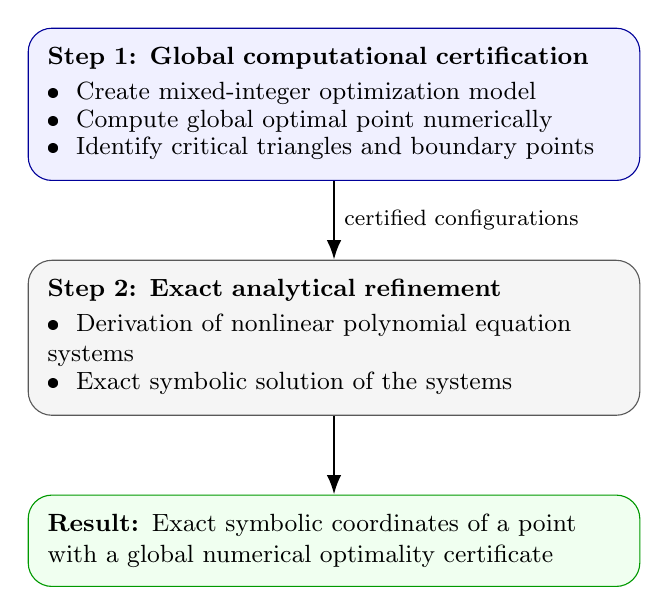
\begin{tikzpicture}[
    font=\small,
    >=Latex,
    node distance=10mm,
    box/.style={
      draw,
      rounded corners=3mm,
      inner sep=7pt,
      text width=0.60\linewidth, % <-- key change: true horizontal shrink
      align=left
    },
    boxA/.style={box, fill=blue!6,  draw=blue!60!black},
    boxB/.style={box, fill=gray!8,  draw=gray!70!black},
    boxC/.style={box, fill=green!6, draw=green!60!black},
    arrow/.style={->, line width=0.9pt},
    dashedarrow/.style={->, line width=0.8pt, dashed}
  ]
  
  %
  \newcommand{\brow}[1]{\textbullet\; #1\\[-1pt]}
  
  \node[boxA] (s1) {
    \textbf{Step 1: Global computational certification}\par\vspace{2pt}
    \begin{tabular}{@{}p{\linewidth}@{}}
      \brow{Create mixed-integer optimization model}
      \brow{Compute global optimal point numerically}
      \brow{Identify critical triangles and boundary points}
    \end{tabular}
  };
  
  \node[boxB, below=of s1] (s2) {
    \textbf{Step 2: Exact analytical refinement}\par\vspace{2pt}
    \begin{tabular}{@{}p{\linewidth}@{}}
      \brow{Derivation of nonlinear polynomial equation systems}
      \brow{Exact symbolic solution of the systems}
    \end{tabular}
  };

  \node[boxC, below=of s2] (result) {
    \textbf{Result:} Exact symbolic coordinates of a point with a global numerical optimality certificate
  };

  
  \draw[arrow] (s1.south) -- node[right, font=\footnotesize] {certified configurations} (s2.north);
  \draw[arrow] (s2.south) -- (result.north);
  
  \end{tikzpicture}
  
\caption{Methodological pipeline of the paper: global computational certification (Step~1), exact analytical refinement (Step~2), yielding points with exact symbolic coordinates and global numerical optimality certificates.}
  \label{fig:pipeline}
  \end{figure}

While due to the recent advances in global mixed-integer nonlinear programming solvers, Step~1 is a standard optimization task, Step~2 is more involved.
The equal-area conditions on the critical triangles form a system of polynomial equations whose unknowns are the free coordinate parameters remaining after boundary constraints and coordinate coincidences have been exploited.
The number~$k$ of these parameters ranges from~$4$ (for $n=5$) to~$8$ (for $n=9$), and we employ three solving strategies, tried in succession.

\begin{enumerate}
\item \emph{Direct symbolic solve.}
For small systems ($k \le 6$, covering $n=5,6,8$), SymPy's symbolic solver produces exact solutions directly, including the detection of the one-parameter family for $n=6$.
\item \emph{Gröbner basis.}
For $n=7$, the solution lies in a cubic extension field; a lexicographic Gröbner basis computation
yields a triangular system from which all coordinates follow by back-substitution through the minimal polynomial $19f^3 - 27f^2 + 11f - 1 = 0$ (see Section~\ref{sec:illustration-n7}).
\item \emph{Numeric-to-symbolic refinement.}
For $n=9$, where $k=8$, neither a direct solve nor a Gröbner basis computation terminates in reasonable time.
Instead, we apply a numeric-to-symbolic approach: from the certified numerical coordinates we first identify the underlying number field~$\mathbb{Q}(\sqrt{65})$ by recognizing~$\sqrt{65}$ in the simplest coordinate, then express all coordinates as elements of this field using SymPy's \texttt{nsimplify} function with the known algebraic extension.
\end{enumerate}

\noindent
The numeric-to-symbolic step involves a risk:
numerical proximity does not guarantee algebraic correctness, since Gurobi's certified values carry only about six significant digits.
For instance, for $n=9$ the spurious expression $\tfrac{19}{166} + \tfrac{3\sqrt{65}}{166} \approx 0.26017$
is numerically indistinguishable from the true value $\tfrac{9}{16} - \tfrac{3\sqrt{65}}{80} \approx 0.26017$
at solver precision, yet only the latter satisfies the equal-area equations.
We therefore verify every candidate solution symbolically by substituting into the full polynomial system.
Any coordinate that fails this check is corrected by fixing the validated coordinates and solving the resulting reduced (and much smaller) subsystem exactly.

The entire pipeline is implemented as a reproducible Python script, available together with all input data in the accompanying repository.\footnote{\url{https://github.com/spiralulam/heilbronn}}

  \subsection{Illustration of the methodology for $n=7$}
  \label{sec:illustration-n7}

  We now illustrate the two-step pipeline on the case $n=7$, for which
  Comellas and Yebra~\cite{comellasyebra2002} heuristically obtained conjectured optimal
  coordinates via simulated annealing followed by a local optimality analysis.
  Global optimality was subsequently proved by Zeng and Chen~\cite{ZengChen2011}, who decomposed the problem into 226 nonlinear optimization subproblems.
  Our approach provides an independent proof and yields simpler coordinate expressions.

  \subsubsection*{Step 1: Global computational certification}

  Running our final MIP model from Section~\ref{sec:final-model} with
  $n=7$, Gurobi terminates after $1.75$ seconds with an optimal value of $\Delta_7 \approx 0.0838590$ and
  the numerical configuration shown in
  Table~\ref{tab:n7-numerical}.

  \begin{figure}[h]
    \centering
    \begin{minipage}[c]{0.3\linewidth}
      \centering
      \begin{tabular}{c c c c}
      \toprule
      Pt & $x$ & $y$ & Edge \\
      \midrule
      $p_1$ & $0$      & $0.1352$ & left edge \\
      $p_2$ & $0.7127$ & $0$      & bottom edge \\
      $p_3$ & $1$      & $0.1808$ & right edge \\
      $p_4$ & $1$      & $1$      & corner \\
      $p_5$ & $0$      & $1$      & corner \\
      $p_6$ & $0.1939$ & $0.4926$ & interior \\
      $p_7$ & $0.7127$ & $0.5839$ & shared $x$ with $p_2$ \\
      \bottomrule
      \end{tabular}
      \captionof{table}{Numerical coordinates returned by Gurobi for $n=7$
       (rounded to four decimal places). Five of the seven points lie on the
       boundary of the unit square.}
      \label{tab:n7-numerical}
    \end{minipage}\hfill
    \begin{minipage}[c]{0.5\linewidth}
      \centering
      \includegraphics[width=\linewidth,trim=35pt 10pt 35pt 10pt,clip]{figs/fig_n7.pdf}
      \captionof{figure}{Optimal configuration for $n=7$
        with its eight critical triangles highlighted.}
      \label{fig:n7-config-step1}
    \end{minipage}
  \end{figure}

  Figure~\ref{fig:n7-config-step1} shows the configuration
  together with its eight critical triangles, which all have areas within
  $5 \times 10^{-7}$ of the optimal value. The ninth-smallest
  triangle area is roughly $0.0948$, leaving a comfortable gap
  of about $13\%$ above the optimum.

  Two structural observations guide the symbolic step that follows:
  \begin{enumerate}
    \item Five of the seven points lie on the boundary
          ($p_4, p_5$ at corners, $p_1$ on the left edge,
           $p_2$ on the bottom edge, $p_3$ on the right edge).
    \item Points $p_2$ and $p_7$ share the same $x$-coordinate,
          suggesting a hidden algebraic relation.
  \end{enumerate}

  \subsubsection*{Step 2: Exact analytical refinement}

  Guided by these observations, we set up a parametric ansatz.
  The boundary structure fixes seven coordinates
  ($x_1 = 0$, $y_2 = 0$, $x_3 = 1$, $x_4 = y_4 = 1$, $x_5 = 0$, $y_5 = 1$),
  and the shared $x$-coordinate of $p_2$ and $p_7$ introduces an additional coupling,
  leaving six unknowns $a, b, c, d, e, f$ (Table~\ref{tab:n7-parametric}).

  \begin{table}[h]
    \centering
    \begin{tabular}{c c c l}
    \toprule
    Pt & $x$ & $y$ & Rationale \\
    \midrule
    $p_1$ & $0$ & $a$ & left edge \\
    $p_2$ & $b$ & $0$ & bottom edge \\
    $p_3$ & $1$ & $c$ & right edge \\
    $p_4$ & $1$ & $1$ & corner \\
    $p_5$ & $0$ & $1$ & corner \\
    $p_6$ & $d$ & $e$ & interior \\
    $p_7$ & $b$ & $f$ & shared $x$ with $p_2$ \\
    \bottomrule
    \end{tabular}
    \caption{Parametric ansatz for $n=7$. Boundary constraints
    fix seven coordinates; the shared $x$-coordinate of $p_2$
    and $p_7$ introduces the coupling $x_7 = b$.}
    \label{tab:n7-parametric}
  \end{table}

  Setting the areas of the eight critical triangles equal yields
  seven polynomial equations in six unknowns.
  A lexicographic Gröbner basis computation eliminates all unknowns
  except~$f$, which must satisfy the irreducible cubic
  \[
    19\,f^{3} - 27\,f^{2} + 11\,f - 1 \;=\; 0.
  \]
  This cubic has three real roots:
  $f_1 \approx 0.1269$,
  $f_2 \approx 0.5839$, and
  $f_3 \approx 0.7103$.
  The first root gives $b = 19f_1^2 - 27f_1 + 10 \approx 6.88 > 1$,
  and the third gives $a = 19f_3^2 - 16f_3 + 3 \approx 1.22 > 1$;
  both violate the unit-square constraint.
  The unique feasible solution corresponds to $f = f_2$.
  Back-substitution through the Gröbner basis yields the
  exact symbolic coordinates in Table~\ref{tab:n7-exact}.

  \begin{table}[h]
    \centering
    \begin{tabular}{c c c}
    \toprule
    Pt & $x$ & $y$ \\
    \midrule
    $p_1$ & $0$ & $19f^{2} - 16f + 3$ \\[6pt]
    $p_2$ & $19f^{2} - 27f + 10$ & $0$ \\[6pt]
    $p_3$ & $1$ & $\displaystyle \frac{-19f^{2} + 10f + 1}{2}$ \\[10pt]
    $p_4$ & $1$ & $1$ \\[6pt]
    $p_5$ & $0$ & $1$ \\[6pt]
    $p_6$ & $-19f^{2} + 8f + 2$ & $57f^{2}-41f+5$ \\[6pt]
    $p_7$ & $19f^{2} - 27f + 10$ & $f$ \\[6pt]
    \bottomrule
    \end{tabular}
    \caption{Exact symbolic coordinates of the optimal seven-point
    configuration, where $f \approx 0.5839$ is the second real root of
    $19f^3-27f^2+11f-1$.}
    \label{tab:n7-exact}
  \end{table}

  The optimal value simplifies to
  \[
    \Delta_7 \;=\; f - \tfrac{1}{2}
              \;\approx\; 0.0838590090\ldots
  \]

  \paragraph{Comparison with Comellas and Yebra~\cite{comellasyebra2002}.}
  The exact coordinates we obtain are notably simpler than those
  reported by Comellas and Yebra, who express
  each coordinate as a degree-two polynomial in a parameter~$z$
  with rational coefficients over denominators~$19$ and~$38$
  and integer numerators as large as~$223$, for
  instance $x_1 = -\tfrac{50}{19}\,z - \tfrac{17}{38}\,z^{2}
  + \tfrac{37}{38}$.
  
%% ============================================================
\section{Optimal solutions for $5\le n\le 9$}\label{sec:solutions}

    \subsection{Software and hardware}

  The models are implemented in Python~3.11 using the Gurobi~13.0 solver interface (\texttt{gurobipy}); the exact symbolic refinements use SymPy~1.14.
  Gurobi's only non-default setting is \texttt{MIPFocus\,=\,2} to prioritise the dual bound.
Computations were carried out on a standard desktop PC equipped with an AMD Ryzen~9 9950X3D processor (16~cores, 4.30\,GHz) and 96\,GB DDR5 RAM.
  
  \subsection{$n=5$: Four critical triangles, $\Delta_5 = \frac{\sqrt{3}}{9}$}
  
  The configuration has four critical triangles.
  Setting these four areas equal yields a system whose unique feasible solution gives the closed-form
  optimal value $\Delta_5 = \sqrt{3}/9 \approx 0.19245$.
  
  \begin{figure}[h]
    \centering
    \begin{minipage}{0.48\linewidth}\centering
      \begin{tabular}{c c c}
      \toprule
      Pt & $x$ & $y$ \\
      \midrule
      $1$ & $0$ & $\frac{1}{3}$ \\[4pt]
      $2$ & $\frac{\sqrt{3}}{3}$ & $0$ \\[4pt]
      $3$ & $1$ & $1 - \frac{\sqrt{3}}{3}$ \\[4pt]
      $4$ & $\frac{2}{3}$ & $1$ \\[4pt]
      $5$ & $0$ & $1$ \\
      \bottomrule
      \end{tabular}
      \captionof{table}{Exact coordinates for $n=5$.}
      \label{tab:n5-exact-compact}
    \end{minipage}\hfill
    \begin{minipage}{0.35\linewidth}\centering
      \includegraphics[width=\linewidth,trim=35pt 10pt 35pt 10pt,clip]{figs/fig_n5.pdf}
      \captionof{figure}{Optimal configuration for $n=5$.}
      \label{fig:n5-config}
    \end{minipage}
  \end{figure}
  
  
  \subsection{$n=6$: Six critical triangles, $\Delta_6 = \frac{1}{8}$}
  
  The configuration has six critical triangles.
  Remarkably, there is a one-parameter family of optimal solutions parameterized by $c \in [0, \tfrac{1}{4}]$,
  all achieving $\Delta_6 = 1/8 = 0.125$. The full distribution of triangle areas is independent of the
  choice of~$c$.
  
  \begin{figure}[h]
    \centering
    \begin{minipage}{0.48\linewidth}\centering
      \begin{tabular}{c c c}
      \toprule
      Pt & $x$ & $y$ \\
      \midrule
      $1$ & $0$ & $c$ \\[4pt]
      $2$ & $\frac{1}{2}$ & $0$ \\[4pt]
      $3$ & $1$ & $\frac{1}{2} - c$ \\[4pt]
      $4$ & $\frac{1}{2}$ & $1$ \\[4pt]
      $5$ & $0$ & $c + \frac{1}{2}$ \\[4pt]
      $6$ & $1$ & $1-c$ \\
      \bottomrule
      \end{tabular}
      \captionof{table}{Exact coordinates for $n=6$, $c\in[0,\tfrac{1}{4}]$.}
      \label{tab:n6-exact-compact}
    \end{minipage}\hfill
    \begin{minipage}{0.35\linewidth}\centering
      \includegraphics[width=\linewidth,trim=35pt 10pt 35pt 10pt,clip]{figs/fig_n6.pdf}
      \captionof{figure}{Optimal configuration for $n=6$.}
      \label{fig:n6-config}
    \end{minipage}
  \end{figure}
  
  
  \subsection{$n=7$: Eight critical triangles, $\Delta_7 = f - \tfrac{1}{2}$}
  
  The detailed derivation for $n=7$ is given in Section~\ref{sec:illustration-n7}.
  The configuration has eight critical triangles, and the exact coordinates are parameterized by
  the root of $19f^3-27f^2+11f-1$ near $0.5839$, yielding $\Delta_7 \approx 0.08386$.
  
  \begin{figure}[h]
    \centering
    \begin{minipage}{0.35\linewidth}\centering
      \begin{tabular}{c c c}
      \toprule
      Pt & $x$ & $y$ \\
      \midrule
      $1$ & $0$ & $19f^{2}-16f+3$ \\[4pt]
      $2$ & $19f^{2}-27f+10$ & $0$ \\[4pt]
      $3$ & $1$ & $\frac{-19f^{2}+10f+1}{2}$ \\[6pt]
      $4$ & $1$ & $1$ \\[4pt]
      $5$ & $0$ & $1$ \\[4pt]
      $6$ & $-19f^{2}+8f+2$ & $57f^{2}-41f+5$ \\[4pt]
      $7$ & $19f^{2}-27f+10$ & $f$ \\
      \bottomrule
      \end{tabular}
      \captionof{table}{Exact coordinates for $n=7$.}
      \label{tab:n7-exact-compact}
    \end{minipage}\hfill
    \begin{minipage}{0.4\linewidth}\centering
      \includegraphics[width=\linewidth,trim=35pt 10pt 35pt 10pt,clip]{figs/fig_n7.pdf}
      \captionof{figure}{Optimal configuration for $n=7$.}
      \label{fig:n7-config}
    \end{minipage}
  \end{figure}
  
  
  \subsection{$n=8$: Twelve critical triangles, $\Delta_8 = -\frac{1}{36}+\frac{\sqrt{13}}{36}$}
  
  The configuration exhibits a point-symmetric
  structure with twelve critical triangles and a unique optimal solution involving $\sqrt{13}$.
  
  \begin{figure}[h]
    \centering
    \begin{minipage}{0.35\linewidth}\centering
      \begin{tabular}{c c c}
      \toprule
      Pt & $x$ & $y$ \\
      \midrule
      $1$ & $0$ & $0$ \\[4pt]
      $2$ & $\frac{1}{6}+\frac{\sqrt{13}}{6}$ & $0$ \\[4pt]
      $3$ & $1$ & $\frac{7}{18}-\frac{\sqrt{13}}{18}$ \\[4pt]
      $4$ & $1$ & $1$ \\[4pt]
      $5$ & $0$ & $\frac{11}{18}+\frac{\sqrt{13}}{18}$ \\[4pt]
      $6$ & $\frac{5}{6}-\frac{\sqrt{13}}{6}$ & $1$ \\[4pt]
      $7$ & $\frac{5}{6}-\frac{\sqrt{13}}{6}$ & $\frac{7}{9}-\frac{\sqrt{13}}{9}$ \\[4pt]
      $8$ & $\frac{1}{6}+\frac{\sqrt{13}}{6}$ & $\frac{2}{9}+\frac{\sqrt{13}}{9}$ \\
      \bottomrule
      \end{tabular}
      \captionof{table}{Exact coordinates for $n=8$.}
      \label{tab:n8-exact-compact}
    \end{minipage}\hfill
    \begin{minipage}{0.4\linewidth}\centering
      \includegraphics[width=\linewidth,trim=35pt 10pt 35pt 10pt,clip]{figs/fig_n8.pdf}
      \captionof{figure}{Optimal configuration for $n=8$.}
      \label{fig:n8-config}
    \end{minipage}
  \end{figure}
  
  
  \subsection{$n=9$: Eleven critical triangles, $\Delta_9 = -\frac{11}{64}+\frac{9\sqrt{65}}{320}$}
  
  The configuration has eleven critical triangles
  and is invariant under reflection in the anti-diagonal $(x,y)\mapsto(1-y,\,1-x)$. The unique optimal solution involves $\sqrt{65}$.
  
  \begin{figure}[h]
    \centering
    \begin{minipage}{0.48\linewidth}\centering
      \begin{tabular}{c c c}
      \toprule
      Pt & $x$ & $y$ \\
      \midrule
      $1$ & $0$ & $1-\frac{\sqrt{65}}{10}$ \\[4pt]
      $2$ & $\frac{3}{8}-\frac{\sqrt{65}}{40}$ & $0$ \\[4pt]
      $3$ & $1$ & $\frac{9}{16}-\frac{3\sqrt{65}}{80}$ \\[4pt]
      $4$ & $\frac{3}{8}-\frac{\sqrt{65}}{40}$ & $1$ \\[4pt]
      $5$ & $0$ & $\frac{5}{8}+\frac{\sqrt{65}}{40}$ \\[4pt]
      $6$ & $\frac{1}{4}+\frac{\sqrt{65}}{20}$ & $\frac{3}{4}-\frac{\sqrt{65}}{20}$ \\[4pt]
      $7$ & $\frac{7}{16}+\frac{3\sqrt{65}}{80}$ & $0$ \\[4pt]
      $8$ & $\frac{\sqrt{65}}{10}$ & $1$ \\[4pt]
      $9$ & $1$ & $\frac{5}{8}+\frac{\sqrt{65}}{40}$ \\
      \bottomrule
      \end{tabular}
      \captionof{table}{Exact coordinates for $n=9$.}
      \label{tab:n9-exact-compact}
    \end{minipage}\hfill
    \begin{minipage}{0.48\linewidth}\centering
      \includegraphics[width=\linewidth,trim=35pt 10pt 35pt 10pt,clip]{figs/fig_n9.pdf}
      \captionof{figure}{Optimal configuration for $n=9$.}
      \label{fig:n9-config}
    \end{minipage}
  \end{figure}


\section{Further observations and research questions}
\label{sec:observations}

\subsection{Growth of the number of critical triangles}
\label{sec:critical-triangle-count}

A structural feature of the optimal configurations worth noting is the number of
critical triangles, i.e., triangles whose area equals the minimum.
Table~\ref{tab:critical-counts} and Figure~\ref{fig:critical-count-plot}
summarize the counts for $n=5,\ldots,9$.

\begin{figure}[h]
  \centering
  \begin{minipage}{0.35\linewidth}\centering
  \begin{tabular}{c c}
  \toprule
  $n$ & Critical triangles \\
  \midrule
  5 & 4 \\
  6 & 6 \\
  7 & 8 \\
  8 & 12 \\
  9 & 11 \\
  \bottomrule
  \end{tabular}
  \captionof{table}{Number of critical triangles for $n = 5, \ldots, 9$.}
  \label{tab:critical-counts}
  \end{minipage}\hfill
  \begin{minipage}{0.55\linewidth}\centering
  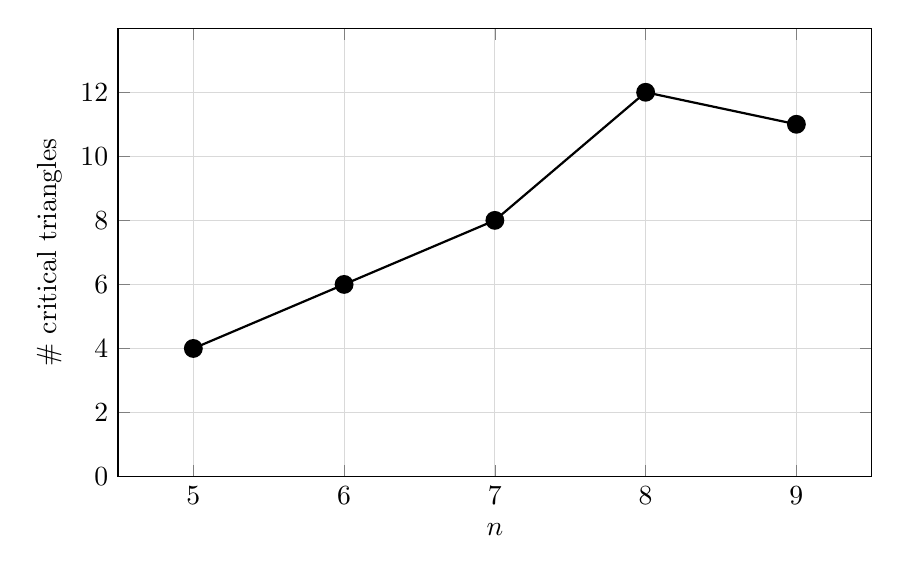
\begin{tikzpicture}
    \begin{axis}[
      width=0.92\linewidth,
      height=0.6\linewidth,
      xlabel={$n$},
      ylabel={\# critical triangles},
      xtick={5,6,7,8,9},
      ytick={0,2,4,6,8,10,12},
      ymin=0, ymax=14,
      xmin=4.5, xmax=9.5,
      grid=major,
      grid style={gray!30},
      mark size=3pt,
      every axis plot/.append style={thick},
    ]
    \addplot[color=black, mark=*, mark options={fill=black}]
      coordinates {(5,4) (6,6) (7,8) (8,12) (9,11)};
    \end{axis}
  \end{tikzpicture}
  \captionof{figure}{Critical triangles as a function of~$n$.}
  \label{fig:critical-count-plot}
  \end{minipage}
\end{figure}

The data suggest a broadly increasing trend, although the decrease from $n=8$
to $n=9$ shows that the growth is not strictly monotone.  A natural question
arises:

\begin{quote}
\emph{Can one establish a nontrivial lower bound on the number of critical
triangles in an optimal Heilbronn configuration as a function of~$n$?}
\end{quote}

Any such bound would have implications for the structure of the polynomial
systems that arise in Step~2 of the framework, since each critical triangle
contributes an equality constraint.  Even a linear lower bound of the form
$\Omega(n)$ would be significant, as it would guarantee that optimal
configurations are constrained by at least as many active area equalities as
there are free coordinate variables.

\begin{remark}
  We thank Oliver Stein for pointing out that the number of critical triangles should be bounded above if the linear independence constraint qualification (LICQ) holds at the optimal solution, since each critical triangle corresponds to an active constraint.  However, we do not know whether LICQ holds for optimal Heilbronn configurations.
\end{remark}


\subsection{Clustering of noncritical triangle areas}
\label{sec:noncritical-clustering}

A second observation concerns the \emph{noncritical}
triangles---those whose area strictly exceeds the minimum.  Inspecting the
degeneracy plots (Figures~\ref{fig: degen n=5} and~\ref{fig: degen n=8}), one
notices that the triangle areas do not spread out continuously but instead
cluster around a small number of distinct values.

For $n=5$, there are only three distinct noncritical area levels beyond the
four critical triangles (see Figure~\ref{fig: degen n=5}).
For $n=8$, the pattern is particularly clear: after the twelve critical
triangles, the remaining $\binom{8}{3} - 12 = 44$ triangle areas visibly
group into a handful of narrow clusters (see Figure~\ref{fig: degen n=8}).
Similar clustering is observed for $n=6$, $n=7$, and $n=9$.

\begin{figure}[h]
  \centering
  \begin{minipage}{0.48\linewidth}\centering
    \includegraphics[width=\linewidth]{figs/degen_plot_n5.pdf}
    \captionof{figure}{Degeneracy plot for $n=5$: all $\binom{5}{3}=10$ triangle areas sorted in ascending order.  Four critical triangles are followed by three clearly separated noncritical area levels.}
    \label{fig: degen n=5}
  \end{minipage}\hfill
  \begin{minipage}{0.48\linewidth}\centering
    \includegraphics[width=\linewidth]{figs/degen_plot_n8.pdf}
    \captionof{figure}{Degeneracy plot for $n=8$: all $\binom{8}{3}=56$ triangle areas sorted in ascending order.  Twelve critical triangles are followed by distinctly clustered noncritical area levels.}
    \label{fig: degen n=8}
  \end{minipage}
\end{figure}

To the best of our knowledge, this clustering phenomenon has not been noted in
the literature.  This suggests a structural rigidity in the extremal configurations
that goes beyond the optimality of the minimum area.

\begin{quote}
\emph{Can one explain the clustering of noncritical triangle areas in optimal
Heilbronn configurations?  In particular, is it possible to show that, for each~$n$,
the $\binom{n}{3}$ triangle areas of an optimal configuration take only
$O(n)$ distinct values?}
\end{quote}

A positive answer would reveal strong hidden symmetries in the optimal
configurations and could considerably simplify the algebraic systems used to
derive exact coordinates.


\section{Outlook and final remarks}\label{sec:outlook}

We have presented an \emph{optimize--then--refine} framework for the
Heilbronn triangle problem on the unit square that combines a
mixed-integer optimization model with exact symbolic computation.
A symmetry-breaking strategy and a product-form determinant
reformulation yield a model that Gurobi solves to certified global
optimality for all $n \le 9$, and the subsequent symbolic step
recovers exact algebraic coordinates from the numerical certificate.

Several directions remain open.
Extending the global certification to $n = 10$ appears within reach
given continued improvements in solver technology and hardware,
but will require substantial computational effort.
On the theoretical side, establishing nontrivial bounds on
the number of critical triangles (Section~\ref{sec:critical-triangle-count})
or explaining the clustering of noncritical triangle areas
(Section~\ref{sec:noncritical-clustering}) would deepen our
understanding of optimal Heilbronn configurations.

More broadly, the two-step methodology illustrated here---global
certification via mixed-integer programming followed by exact
coordinate recovery through computer algebra---is applicable
to other packing and covering problems in discrete geometry
where the conjectured optimal configurations involve
algebraic numbers of moderate degree.

\section*{Acknowledgments}
We thank Erich Friedman for kindly sharing the previously unpublished
best-known configurations of Peter Karpov ($n=13,15$) and Mark Beyleveld
($n=14,16$) reproduced in Appendix~\ref{app:best-known}.

\printbibliography

\appendix\label{appendix}

\section{Best-known configurations for $10\le n\le 16$}
\label{app:best-known}

For completeness, we collect the best-known configurations for $10\le n\le 16$.
Those for $n=10$ and $n=12$ are due to Comellas and Yebra~\cite{comellasyebra2002},
the one for $n=11$ to Goldberg~\cite{goldberg1972maximizing}, and the remaining
ones to Peter Karpov ($n=13,15$) and Mark Beyleveld ($n=14,16$), all unpublished.
The exact coordinates are listed in
Tables~\ref{tab:bestknown}--\ref{tab:bestknown-1516}; the parameters appearing in
the $n=10$ and $n=12$ entries are defined next.

\begin{itemize}
  \item For $n=10$, let $z = \frac{3}{4} - \frac{(63+8\sqrt{62})^{1/3}}{12} - \frac{1}{12(63+8\sqrt{62})^{1/3}} \approx 0.3156$,
$x = z/2$, and $y = 1-3z+2z^2$.
\item For $n=12$, let $x = 1 - \frac{(27+3\sqrt{57})^{2/3}+6}{6(27+3\sqrt{57})^{1/3}} \approx 0.1154$
and $y = 2x^2-3x+\frac{1}{2}$.
\end{itemize}

\begin{table}[ht]
\centering
\caption{Best-known configurations for $n=10,\ldots,16$.
The configurations for $n=10,12$ are due to Comellas and Yebra~\cite{comellasyebra2002},
$n=11$ to Goldberg~\cite{goldberg1972maximizing},
$n=13,15$ to Peter Karpov (unpublished),
and $n=14,16$ to Mark Beyleveld (unpublished).}
\label{tab:bestknown}
{\small
\begin{tabular}{r c@{\hskip 6pt} c @{\hskip 14pt} r c@{\hskip 6pt} c @{\hskip 14pt} r r@{\hskip 6pt} r}
\toprule
\multicolumn{3}{c}{$n=10$} & \multicolumn{3}{c}{$n=11$} & \multicolumn{3}{c}{$n=12$} \\
\# & $x$ & $y$ & \# & $x$ & $y$ & \# & $x$ & $y$ \\
\midrule
$0$ & $x$ & $0$       & $0$ & $1/3$ & $0$     & $0$ & $x$ & $0$ \\
$1$ & $1{-}y$ & $0$    & $1$ & $2/3$ & $0$     & $1$ & $1{-}x$ & $0$ \\
$2$ & $0$ & $x$        & $2$ & $0$ & $2/9$     & $2$ & $0$ & $x$ \\
$3$ & $1$ & $y$        & $3$ & $1$ & $2/9$     & $3$ & $1$ & $x$ \\
$4$ & $1{-}z$ & $z$    & $4$ & $1/3$ & $4/9$   & $4$ & $1/2$ & $y$ \\
$5$ & $z$ & $1{-}z$    & $5$ & $2/3$ & $4/9$   & $5$ & $y$ & $1/2$ \\
$6$ & $0$ & $1{-}y$    & $6$ & $0$ & $2/3$     & $6$ & $1{-}y$ & $1/2$ \\
$7$ & $1$ & $1{-}x$    & $7$ & $1$ & $2/3$     & $7$ & $1/2$ & $1{-}y$ \\
$8$ & $y$ & $1$        & $8$ & $1/2$ & $7/9$   & $8$ & $0$ & $1{-}x$ \\
$9$ & $1{-}x$ & $1$    & $9$ & $1/6$ & $1$     & $9$ & $1$ & $1{-}x$ \\
   &     &             & $10$ & $5/6$ & $1$    & $10$ & $x$ & $1$ \\
   &     &             &      &       &        & $11$ & $1{-}x$ & $1$ \\
\midrule
\multicolumn{3}{c}{$\Delta_{10} \ge \tfrac{5}{8}z^2 {-} \tfrac{1}{2}z^3 \approx 0.04654$}
& \multicolumn{3}{c}{$\Delta_{11} \ge 1/27 \approx 0.03704$}
& \multicolumn{3}{c}{$\Delta_{12} \ge \tfrac{1}{4}x {+} \tfrac{1}{2}xy {-} \tfrac{1}{2}x^2 \approx 0.03260$} \\
\bottomrule
\end{tabular}}
\end{table}

\begin{table}[ht]
\centering
\caption{Best-known configurations for $n=13$ and $n=14$.}
\label{tab:bestknown-1314}
{\small
\begin{tabular}{r r@{\hskip 6pt} r @{\hskip 14pt} r r@{\hskip 6pt} r}
\toprule
\multicolumn{3}{c}{$n=13$} & \multicolumn{3}{c}{$n=14$} \\
\# & $x$ & $y$ & \# & $x$ & $y$ \\
\midrule
0 & 0.964815 & 0.087630 & 0 & 0.077620 & 0 \\
1 & 0 & 1               & 1 & 0.922380 & 1 \\
2 & 0.896939 & 0.902546 & 2 & 0.922380 & 0 \\
3 & 0.761346 & 0.441996 & 3 & 0.077620 & 1 \\
4 & 0.655161 & 1         & 4 & 0 & 0.186886 \\
5 & 0.748551 & 0         & 5 & 1 & 0.813114 \\
6 & 0 & 0.099250         & 6 & 1 & 0.186886 \\
7 & 1 & 0.461332         & 7 & 0 & 0.813114 \\
8 & 0.328490 & 0.633357 & 8 & 0.292333 & 0.321345 \\
9 & 0.087939 & 0.614507 & 9 & 0.707667 & 0.678655 \\
10 & 0.345014 & 0.901507 & 10 & 0.707667 & 0.321345 \\
11 & 0.087938 & 0         & 11 & 0.292333 & 0.678655 \\
12 & 0.500181 & 0.149235 & 12 & 0.5 & 0.138278 \\
   &          &           & 13 & 0.5 & 0.861722 \\
\midrule
\multicolumn{3}{c}{$\Delta_{13} \ge 0.02702$}
& \multicolumn{3}{c}{$\Delta_{14} \ge 0.02430$} \\
\bottomrule
\end{tabular}}
\end{table}

\begin{table}[ht]
\centering
\caption{Best-known configurations for $n=15$ and $n=16$. All coordinates for $n=16$ are rational.}
\label{tab:bestknown-1516}
{\small
\begin{tabular}{r r@{\hskip 6pt} r @{\hskip 14pt} r r@{\hskip 6pt} r}
\toprule
\multicolumn{3}{c}{$n=15$} & \multicolumn{3}{c}{$n=16$} \\
\# & $x$ & $y$ & \# & $x$ & $y$ \\
\midrule
0 & 0.934094 & 1         & 0 & $2/31$ & $0$ \\
1 & 0.287119 & 0.302829 & 1 & $29/31$ & $1$ \\
2 & 0.342286 & 0.701349 & 2 & $23/31$ & $0$ \\
3 & 0.963064 & 0.095730 & 3 & $8/31$ & $1$ \\
4 & 0.066630 & 0.633568 & 4 & $0$ & $10/33$ \\
5 & 0.648909 & 0         & 5 & $1$ & $23/33$ \\
6 & 0.277707 & 1         & 6 & $1$ & $2/33$ \\
7 & 0.066641 & 0         & 7 & $0$ & $31/33$ \\
8 & 0.589972 & 0.272487 & 8 & $8/31$ & $4/11$ \\
9 & 0.603055 & 0.928222 & 9 & $23/31$ & $7/11$ \\
10 & 0.895664 & 0.684290 & 10 & $10/31$ & $2/33$ \\
11 & 0 & 0.192215        & 11 & $21/31$ & $31/33$ \\
12 & 0.670814 & 0.614942 & 12 & $21/31$ & $10/33$ \\
13 & 0 & 0.924975        & 13 & $10/31$ & $23/33$ \\
14 & 1 & 0.399875        & 14 & $29/31$ & $4/11$ \\
   &   &                 & 15 & $2/31$ & $7/11$ \\
\midrule
\multicolumn{3}{c}{$\Delta_{15} \ge 0.02111$}
& \multicolumn{3}{c}{$\Delta_{16} \ge 7/341 \approx 0.02053$} \\
\bottomrule
\end{tabular}}
\end{table}

\end{document}
